\chapter{Háttérinformációk}

\section{A \emph{syslog-ng}-ről}

\subsection{A fejlesztéshez használt technológiák}

Ebben az alszekcióban szeretném bemutatni azokat az eszközöket, amelyek a fejlesztéshez nap mint nap
használunk.

\begin{description}
    \item[JIRA] {Az Atlassian által fejlesztett, elsősorban hibajegyek kezelésére használatos
        szoftver. Esetünkben a \emph{VersionOne}-t váltotta le.}
    \item[Zorp Build System (ZBS)] {A ZBS egy házon belül fejlesztett eszköz, célja a forráskódból
        a telepíthető binárisok, csomagok előállítása, azaz elfedni a különböző platformok (CPU
        architektúrák, futtató operációs rendszer, stb.) közötti fordítási és csomagolási
        folyamatokban lévő különbségeket. Mivel vannak olyan támogatott platformok, amelyek
        kevésbé szokványos hardvereket igényelnek, és egy ilyen gépen nem történhet párhuzamosan
        több fordítás, ezért a ZBS-nek ezeket az erőforrásokat is kezelnie kell. }
    \item[ZTS] {asd }
    \item[git] {A git már egy nagy múltra visszatekintő (először 2005-ben adták ki), eredetileg a
        Linux kernel fejlesztését segítő, elosztott verziókezelő rendszer. Elosztottságának
        köszönhetően a nyílt forráskódú szoftverek világában az egyik legnagyobb mértékben
        adoptált, köztük a \emph{syslog-ng} fejlesztésénél is ezt használjuk mindkét változatában.
        (Kereskedelmi termékek fejlesztésénél ez annyira nem jellemző, nekünk viszont erősen
        ajánlott azért, hogy a két változat közötti kódmozgatás gördülékenyebb legyen.)}
    \item[GitHub] {Habár egy egyszerű tárhelynek tűnhet csupán, mégis az általa adott
        többletszolgáltatások a közösség által fejlesztett syslog-ng központi elemévé tette.
        Ilyen többletszolgáltatás a \emph{forkok} könnyű kezelése, a beépített hibajegykezelő,
        a \emph{pull request}-ek könnyű kezelése (azaz a GitHub-on lévő forkomból pár
        kattintással tudok kontribúciót küldeni az \emph{upstream repository}-ba), és a könnyű
        bővíthetősége, például lektorálást segítő eszközökkel, \emph{Continous Integration}-t
        megvalósító eszközökkel, statikus kódanalízist biztosító eszközökkel.
        Természetesen a névválasztás nem véletlen, nagyban épít a korábban említett \emph{git}
        verziókezelőre.}
\end{description}

\subsection{A fejlesztés során felmerülő problémák}

A teljesség igénye nélkül listázzuk a fejlesztést nehezítő, olykor értékes fejlesztői időt pazarló
problémákat:
\begin{itemize}
    \item Lassú lektorálási folyamat a közösség által fejlesztett változatban.
\end{itemize}
Sikerült ennek néhány komponensét azonosítani, amelyek:

\begin{itemize}
    \item nincs a kód automatikusan formázva.
\end{itemize}
Érdekesség, hogy a \emph{CVE-2014-1266}\cite{cve20141266}, közismertebb nevén \emph{goto fail;} sérülékenységet egy
egyszerű \emph{code beautifier} figyelemfelkeltőbbé tette volna azáltal, hogy a tabulálásokat
(pontosabban fogalmazva \emph{indent}álásokat) helyessé tette volna.

\begin{itemize}
    \item Meredek tanulási görbe a belső eszközök használatánál:
\end{itemize}
, amelyből következik, hogy
\begin{itemize}
    \item a saját eszközök (főként: ZBS) belső működéséhez kevesen értenek.
\end{itemize}
Ezért ennek a területnek definíció szerint alacsony a \emph{busz faktora}, amely hosszabb távon
nézve kockázatos mind biztonsági (szélsőséges esetben egy ember ismer egy rendszert igazán, így az
ő módosításainak lektorálása nem hatékony), mind termelékenységi szempontból (hiszen ilyenkor
ez az ember szűk keresztmetszetként viselkedik).

\begin{itemize}
    \item Törékeny fejlesztési infrastuktúra.
\end{itemize}
Ez leginkább abban mutatkozik meg, hogy vannak olyan fejlesztői gépek, amelyeknél azok létrehozási
lépései elvesztek, illetve az idők során az azon végzett módosítások nem lettek megfelelően
dokumentálva. Amennyiben ez a fejlesztés szempontjából egy kritikus gép, belátható, hogy az egy
időzített bombaként viselkedik a rendszerben. Ennek a problémának egy tipikus áthidalása, ha az
adott gépről létezik visszaállítható biztonsági mentés, hiszen ekkor egy jól működő állapotra
visszaállhatunk, de az esetleges korszerűsítés (például frissebb operációs rendszerre való átállás)
még problémákat jelenthet.

Úgy gondoljuk, hogy ezek kijavítása ugyan kezdetben sok erőforrást igényelhetnek, de a későbbiekben
olyan mértékben egyszerűsítik a fejlesztők életét, hogy ez a befektetés megtérül.

\section{További termékbiztonságot elősegítő módszerek vizsgálata}

Időközben magasabb vezetési szintről felmerült az igény, hogy legyünk tisztában a termékeink
biztonsági állapotával, ezért erősen ajánlott egy olyan módszer kiválasztása, amely alkalmazható
kész \emph{appliance} termékre, és szoftverre egyaránt.

Habár a használt értékelő keretrendszer kiválasztása még a szakdolgozat létrejötte előtt megtörtént,
mégis érdemesnek tartom a hasonló, termékbiztonságot elősegítő módszerek bemutatását. Az egyes
megközelítések feltérképezéséhez és megvizsgálásához remek kiindulási alapot adott az alábbi
publikáció:
\url{http://citeseerx.ist.psu.edu/viewdoc/download?doi=10.1.1.132.4843&rep=rep1&type=pdf}.

\subsection{Attack trees}

Az \emph{Attack trees} egy olyan módszer, amellyel egy adott támadást elemezhetünk egyszerűen, egy
faként reprezentálva az alábbi szabályok mentén:
\begin{enumerate}
    \item A fa gyökerében az az esemény áll, amely bekövetkezésekor a támadást sikeresnek tekintjük.
    \item A szülő és a gyerek eseménye között az a kapcsolat, hogy a szülő eseménye akkor, és csak
        akkor következik be, ha a gyerek eseménye is.  Összekapcsolt gyerekek esetén akkor és csak
        akkor, ha mindegyik gyerek eseménye bekövetkezett.
\end{enumerate}
Miután megtaláltuk az eseményeink függőségeit (pontosabban a további felbontásnak már nem lenne
értelme), lehetőségünk van ezeket különféle szempontokból elemezni, például az alábbi szempontok
mentén:
\begin{itemize}
    \item Lehetséges-e egyáltalán az esemény bekövetkezése?
    \item Mekkora költséggel jár előidézni az eseményt?
    \item Mekkora költséggel jár megelőzni az eseményt?
    \item Szükséges-e különleges felszerelés az előidézéshez?
\end{itemize}

\begin{figure}[h]
    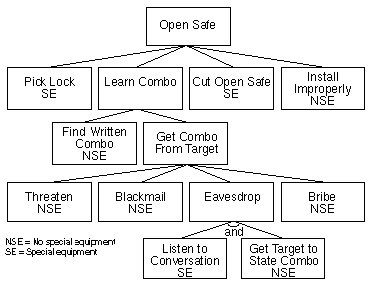
\includegraphics[height=0.4\textheight]{figures/attacktrees.png}
    \centering
    \caption{Példa }
\end{figure}

Az alábbi szempontok segíthetnek eldönteni, hogy megéri-e foglalkozni a védelem kialakításával,
szem előtt tartva, hogy mit feltételezünk a támadóról.

Habár a módszer kellően könnyedén értelmezhető (hiszen csupán egy fát használ) és könnyedén
alkalmazható, számunkra kevésbé használható, hiszen
\begin{itemize}
    \item{nem kellően széleskörű,}
    \item{megoldásokat egyáltalán nem szolgáltat,}
    \item{a teljesség nem garantált.}
\end{itemize}

\subsection{Abuse/Misuse cases}

Az \emph{Misuse cases} az ismert \emph{use case} diagramnak a kifordított változata, azaz ahelyett,
hogy azt modelleznénk, hogy egy adott szereplő milyen tevékenységeket végezhet el, itt inkább azt
modellezzük, hogy egy rosszindulatú szereplő milyen tevékenységeket végezne el, azaz
meghatározhatjuk azokat a tevékenységeket, amelyeket a \emph{rendszernek tiltania kellene}.

\begin{figure}[h]
    \centering
    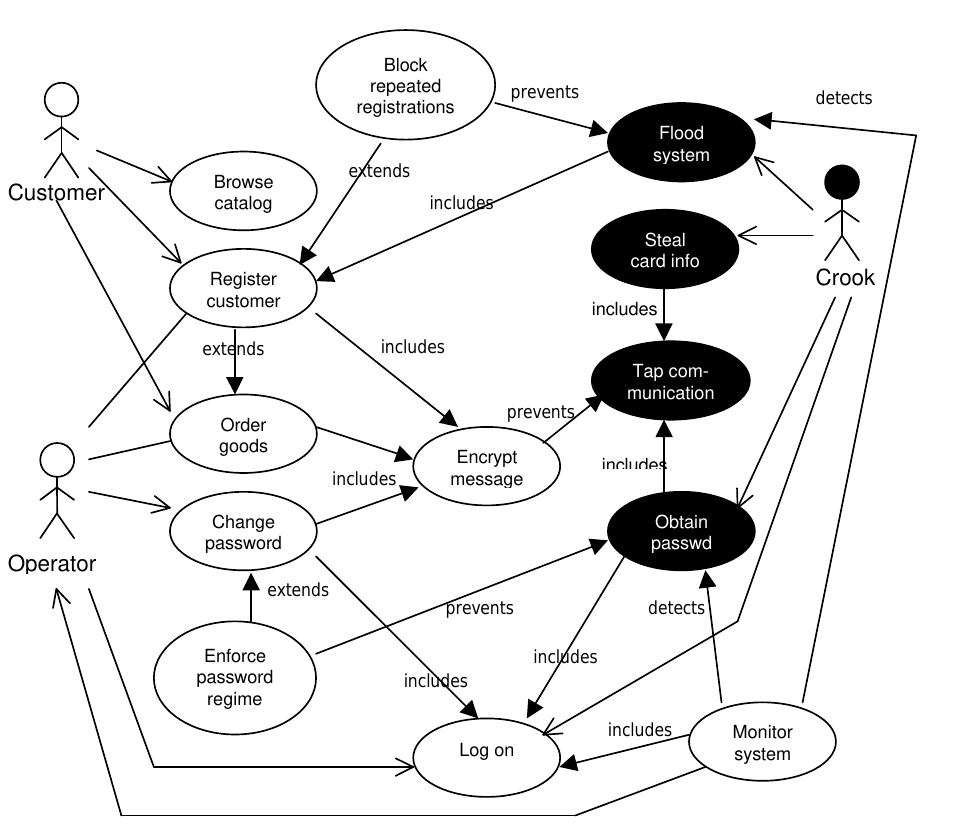
\includegraphics[width=\textwidth, height=0.5\textheight, keepaspectratio]{figures/misusecase.png}
\end{figure}

\FloatBarrier
% \subsection{ISO 27000-as család}
% \subsubsection{ISO 27001:2013}
% Ellentétben a korábbi megközelítésekkel, az \emph{ISO 27001}-es szabvány 
% 
% Habár elsőre nem tűnik indokoltnak a megemlítése, elég csupán arra gondolnunk, hogy egy termék
% fejlesztésekor elvárhatjuk, hogy a belső infrastruktúránk biztonságos.  Ahogy a cég (és ezzel együtt
% az infrastruktúra) növekszik, egyre inkább fontossá válik egy olyan kész keret bevezetése, amelyet
% felhasználva biztonságosabb rendszert építhetünk.

\section{Common Criteria}

A Common Criteria eredetileg egy olyan kezdeményezés volt, amely a már meglévő biztonsági
értékeléseket (köztük az európai \emph{Information Technology Security Evaluation Criteria (ITSEC)},
a \emph{Trusted Computer System Evaluation Criteria (TCSEC)}-t, és a
\emph{Canadian Trusted Computer Product Evaluation Criteria (CTCPEC)}-t) kívánta egyesíteni, ezáltal
elkerülve a korábbi ismételt kiértékeléseket egy nemzetközi piacra szánt termék esetén.  Az első
végleges változatát 1994-ben adták ki, 1999-ben a \emph{2.1}-es verziója az \emph{ISO/IEC 15408}-as
szabvánnyá vált. Legfrissebb változata a \emph{3.1 rev. 4}-es.

\subsection{Terminológia}

\begin{description}
    \item[Target of Evaluation (TOE)] {Az az entitás, amelyre a \emph{Common Criteria} által
        megfogalmazott követelmények teljesülését vizsgáljuk. Esetünkben ez a \emph{syslog-ng}-re,
        mint szoftvercsomagra vonatkozik.}
    \item[Protection Profile (PP)] { Az implementációfüggetlen leírása egy adott TOE-típus
        biztonsági követelményeinek, tulajdonságainak. }
    \item[Security Target (ST)] { Az implementációfüggő leírása az adott TOE biztonsági
        tulajdonságainak. Tartalmazza többek között a lehetséges fenyegetettségeket, feltétlezéseket
        a TOE környezetével kapcsolatban. Egy \emph{Security Target} megvalósíthat több
        \emph{Protection Profile}-t, azaz a \emph{PP} kvázi az \emph{ST} sablonjaként szolgál. }
    \item[Secutiry Functional Requirement (SFR)] { }
    \item[Security Assurance Requirement (SAR)] { Annak egy szabványosított leírása, hogy milyen
        intézkedéseket tettünk a fejlesztés során annak érdekében, hogy a \emph{TOE} teljesítse az
        \emph{SFR}-eket.}
    \item[Evaluation Assurance Level (EAL)]{Evaluation Assurance Level - a követelmények
        szigorúságának számszerűsített értéke, lásd később.}
\end{description}

\subsection{Az egyes EAL szintek jelentései}

Az \emph{Evaluation Assurance Level} (továbbiakban: EAL) egy egytől hétig tartó skálán egyre nagyobb
nyújt, pontosabban a magasabb szinteknél szigorúbb elvárásoknak kell megfelelni. A szigorúbb
elvárásoknak való megfelelőség óhatatlanul magasabb költségekkel is járhat, így az elérni kívánt
szint meghatározásánál figyelembe kell venni, hogy milyen előnyökkel és költségekkel jár annak
elérése.

\subsubsection{EAL1 - funkcionálisan tesztelt}
Ennek a szintnek az a célja, hogy a biztosítsuk azt, hogy a vizsgált termék funkcionalitása a
biztosított dokumentációval összhangban legyen. Éppen ezért a kiértékelés során jellemzően annyi
információt használunk fel, mint a termék egy vásárlója, ezáltal akár a vásárló is megbizonyosodhat
a specifikáció betartásáról, a fejlesztőktől teljesen függetlenül.

Az esetleges biztonsági kockázatokat még nem tekintjük itt komolynak, és a biztonsági funkcionális
követelményeket csupán deklaráljuk ahelyett, hogy azok feltételezések és fenyegetettségekből
kerülnének levezetésre.

\subsubsection{EAL2 - strukturálisan tesztelt}
Az előző szinthez képest már magasabb szintű biztosítást nyújtunk a szint megvalósításával azáltal,
hogy a dokumentációkban nyújtunk tervezési információt, és megosztjuk az egyes tesztek eredményeit.
A biztosított dokumentációk területén annyi változás történt, hogy a specifikációnak itt már
részletesebbnek kell lennie, tartalmaznia kell egy áttekintést a vizsgált termék architektúrájáról,
továbbá demonstrációt, hogy a vizsgált termék képes ellenállni korlátozott kapacitású támadó ellen.

\subsubsection{EAL3 - módszeresen tesztelt és ellenőrzött}
Ez a szint lehetővé teszi, 
Annak érdekében, hogy megérthessük a TOE biztonsági működését, a biztosított dokumentációnak
tartalmaznia kell az előző szintnél részletesebb architekturális leírást TOE-ről.
További előrelépést jelent az \emph{EAL2}-höz képest, hogy
\begin{itemize}
    \item a biztonsági funkcionalitást átfogóbban kell tesztelni, azaz ott a tesztlefedettségnek
        nagyobbnak kell lennie, és
    \item olyan folyamatokat és szabályozókat kell bevezetni, amelyekkel minimalizálni tudjuk a
        termékfejlesztés közbeni szabotázs lehetőségét.
\end{itemize}

\subsubsection{EAL4 - módszeresen tervezett, tesztelt és lektorált}

Az \emph{EAL3}-hoz képest úgy növeli a bizonyosságot, hogy:
\begin{itemize}
    \item a TOE biztonsági funkcionalitásához kapcsolodó implementáció reprezentációját
        (azaz a forráskódját) biztosítani kell,
    \item az előző szinten bevezetett szabotázst megakadályozó mechanizmusokat/folyamatokat
        fejleszteni kell, főként erősebb automatizálással,
    \item a TOE felépítésének modulárisnak kell lennie, és erről egy átfogó képet kell adni, és
    \item az interfész specifikáltságának teljesnek kell lennie.
\end{itemize}

Általában az \emph{EAL4} szint az a legmagasabb szint elérendő szint, amely egy már meglévő termék
esetén is még gazdaságos lehet, mivel habár szigorú, speciális tudást kevésbé igényel.

\subsubsection{EAL5 - félformálisan tervezett és tesztelt}
\begin{description}
    \item[félformális]{Olyan korlátozott szintaxisú nyelvezet, amelynél a szemantika előre
        definiált, például ilyen lehet az UML osztálydiagramja.}
\end{description}
\subsubsection{EAL6 - formálisan verifikált}
\subsubsection{EAL7 - formálisan verifikált}
\begin{description}
    \item[formális]{Olyan félformális nyelvezet, melynek szemantikája megalapozott matematikai
        koncepciókon alapul.}
\end{description}

